\tikzset{>=latex} % for LaTeX arrow head
\colorlet{BFcol}{red!60!black}
\tikzstyle{force}=[->,thick,BFcol]
\def\a{2.1}
\def\F{1.0}

\tikzset{
  pics/magnet/.style={ %args={#1}
    code={
      \def\h{0.8}
      \coordinate (-N) at (0,\h);
      \coordinate (-S) at (0,-\h);
      \draw[pic actions,thick,top color=red!60,bottom color=red!90,shading angle=20]
        (-0.8*\h/2,0) rectangle ++(0.8*\h,\h);
      \draw[pic actions,thick,top color=blue!60,bottom color=blue!90,shading angle=20]
        (-0.8*\h/2,0) rectangle ++(0.8*\h,-\h);
      \node[pic actions] at (0, \h/2) {\textbf{N}};
      \node[pic actions] at (0,-\h/2) {\textbf{S}};
  }},
  pics/nail/.style={
    code={
      \def\t{0.08}
      \def\L{1.2}
      \def\w{0.16}
      \def\h{0.08}
      \coordinate (-N) at (\L/2+\h,0);
      \coordinate (-S) at (0,0);
      \draw[pic actions,thick,top color=black!20,bottom color=black!50,shading angle=20]
        (\L/2,\t/2) --++ (0,-\t) --++ (-\L,0) --++ (-0.14*\L,\t/2) --++ (0.14*\L,\t/2) -- cycle;
      \draw[pic actions,thick,top color=black!20,bottom color=black!50,shading angle=20]
        (\L/2,-\w/2) rectangle ++(\h,\w) -- cycle;
  }}
}

% ATTRACTING MAGNETS SN - SN




% REPELLING MAGNETS SN - NS


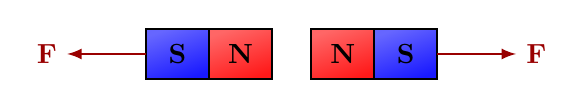
\begin{tikzpicture}
  \pic[rotate=-90] (L) at (-\a/2,0) {magnet};
  \pic[rotate=90] (R) at (\a/2,0) {magnet};
  \draw[force] (L-S) --++ (-\F,0) node[left] {$\mathbf{F}$};
  \draw[force] (R-S) --++ (+\F,0) node[right] {$\mathbf{F}$};
\end{tikzpicture}
